\section{Sprint 3: Corrección de incidencias}%Corrección de issues 

\subsection{Descripción}
%navbar responsive
En este sprint se corregirán los errores detectados en las pruebas realizadas con anterioridad, en los siguientes sprints:
    \begin{itemize}
    \item \textbf{Sprint 1}: Generación de perfil de datos personales.
    \item \textbf{Sprint 2}: Creación y gestión de mediciones.
    \end{itemize}
    
Cabe destacar que sólo se documentarán aquellas correcciones que se refieran a las funcionalidades relevantes seleccionadas, acerca de la ``Carga y muestra de mediciones''

Se desarrollarán las interfaces que permiten mostrar las gráficas de las mediciones de un usuario.
Además, se realizarán las validaciones necesarias para que el sistema funcione correctamente.

Es importante indicar que, en este sprint, el equipo se presentó y quedó como finalista en el \textbf{concurso ``Premio a la Innovación Tecnológica''}, organizado por el Polo IT de Buenos Aires, por lo cual se debió organizar y preparar la presentación a exponer.
En este sentido, se realizó un vídeo de presentación, una página web, tarjetas de contacto, y se preparó un \textbf{\textit{elevator pitch}} para convencer al público y presentarles el proyecto en un período muy corto de tiempo.


\subsection{User Stories relacionados}
La \textbf{Tabla \ref{US-Sprint3}} indica las características de cada \textit{user story} relacionado, y servirá como guía fundamental para el desarrollo completo del sprint.

\begin{table}[h]
    \centering
	\begin{tabular}{|m{1.5cm}|m{11.5cm}|}
	\hline
        \multicolumn{1}{|c|}{\textbf{ID}} &
        \multicolumn{1}{c|}{\textbf{Enunciado de la historia}} \\          
    \hline
        \textbf{US-\ref{evitarPerdidas}} & Como \textbf{paciente}, quiero añadir al sistema los estudios realizados, para evitar posibles pérdidas.\\
     \hline 
        \textbf{US-\ref{cargaCentroSalud}} & Como \textbf{paciente}, quiero que los sistemas de salud existentes puedan cargar sus resultados directamente en mi carpeta de salud, para centralizar mi información. \\
      \hline 
        \textbf{US-\ref{categorizarEstudios}} & Como \textbf{paciente}, quiero categorizar mis estudios por rama de medicina, para lograr una mejor organización y navegabilidad en el sistema. \\
       \hline 
        \textbf{US-\ref{infoPaciente}} & Como \textbf{laboratorio}, quiero cargar información de un paciente en su cuenta, para ahorrarle las molestias de volver. \\
    \hline 
	    \textbf{US-\ref{graficaParaPaciente}} & Como \textbf{paciente}, quiero ver gráficas que resuman mi información en particular, para poder ver mis cambios a lo largo de la historia.\\
    \hline        
        \textbf{US-\ref{graficaParaMedico}} & Como \textbf{médico}, quiero ver gráficas que resuman la información de un paciente, para poder ver sus cambios a lo largo de la historia y así apoyar la toma de decisiones y el diagnóstico.\\
    \hline
    \end{tabular}
    \caption{Listado de \textit{User Stories} relacionados.}
    \label{US-Sprint3}
\end{table}


\subsection{Planificación}

\subsubsection{Período de realización}
\begin{itemize}
    \item \textbf{Inicio}: 7 de julio del 2015.
    \item \textbf{Fin}: 16 de agosto del 2015.
\end{itemize}

\subsubsection{Sprint Backlog}

En la \textbf{Tabla \ref{Backlog-Sprint3}} se detalla el \textbf{Sprint Backlog} actual, indicando las tareas planificadas y efectuadas, en conjunto con el área a cargo de la misma, el responsable de la tarea, su descripción, \textit{user stories} relacionados, y tiempo de ejecución.

\begin{sidewaystable}
    \centering
		\begin{tabular}{|m{3cm}|m{4cm}|m{6cm}|>{\centering\arraybackslash}m{1.5cm}|>{\centering\arraybackslash}m{2cm}|}
			\hline
			\multicolumn{1}{|c|}{\textbf{Área a cargo}} &
			\multicolumn{1}{c|}{\textbf{Responsable}} &        
			\multicolumn{1}{c|}{\textbf{Tarea}} &
			\textbf{US} &
			\textbf{Tiempo}\\
			\hline
				Documentación& Michael Manganiello & Trabajo práctico integrador nº 2: ``Planificación de proyectos informáticos''. & N/A & 17 horas \\ \hline
				Documentación & Iván Terreno & Trabajo práctico integrador nº 2: ``Planificación de proyectos informáticos''. & N/A & 17 horas \\ \hline
				Documentación & Yanina Morales & Trabajo práctico integrador nº 2: ``Planificación de proyectos informáticos''. & N/A & 17 horas \\ \hline
				Documentación& Franco Canizo & Trabajo práctico integrador nº 2: ``Planificación de proyectos informáticos''. & N/A & 17 horas \\ \hline
				Presentaciones & Todos & Postulación del proyecto a BAIT 2015. & N/A & 4 horas \\ \hline
				Presentaciones & Todos & Preparación de la presentación para BAIT 2015. & N/A & 15 horas \\ \hline        
				Front-end& Yanina Morales & Creación de validadores y mensajes de alerta. & US-\ref{evitarPerdidas} \newline US-\ref{cargaCentroSalud} \newline US-\ref{infoPaciente}& 10 horas \\ \hline   
				Front-end& Yanina Morales & Generación de pruebas automatizadas para la carga y muestra de datos personales. & US-\ref{evitarPerdidas} \newline US-\ref{categorizarEstudios} & 10 horas \\ \hline  
				Front-end& Iván Terreno & Generación de pruebas automatizadas para la carga y muestra de mediciones. & US-\ref{evitarPerdidas} \newline US-\ref{graficaParaMedico} \newline US-\ref{graficaParaPaciente} & 10 horas \\ \hline  	              
		\end{tabular}
	\caption{\textit{Sprint Backlog}: Listado de tareas planificadas y efectuadas.}
	\label{Backlog-Sprint3}
\end{sidewaystable}

\subsubsection{Actividades de integración}

Las \textbf{Figuras \ref{pull_request_sprint_3}} y \textbf{\ref{3-PR_back}} detallan las peticiones de integración realizadas por el Front-end sobre el repositorio del proyecto, durante el plazo comprendido por el sprint actual.

\begin{figure}[h]
  \centering
  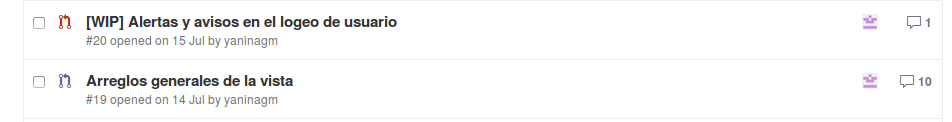
\includegraphics[width=.8\textwidth]{img/3-PR_1_front}
  \caption{Pull requests realizados en el sprint 3, primera parte.}
  \label{pull_request_sprint_3}
\end{figure}
\begin{figure}[h]
  \centering
  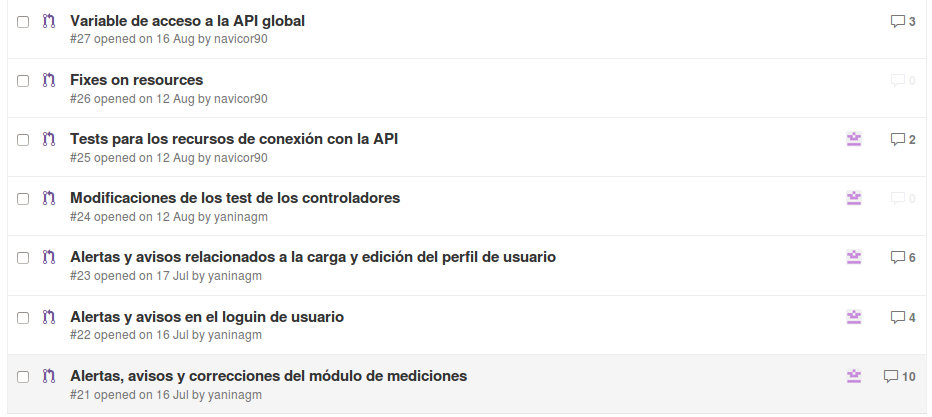
\includegraphics[width=.8\textwidth]{img/3-PR_2_front}
  \caption{Pull requests realizados en el sprint 3, segunda parte.}
  \label{3-PR_back}
\end{figure}

\subsection{Modelo de datos}
\label{3-clases_involucradas}

En la \textbf{Figura \ref{relacion_tipo}} se detalla el diagrama de clases \textit{parcial}, utilizado durante el sprint actual.

\begin{figure}[h]
	\centering
	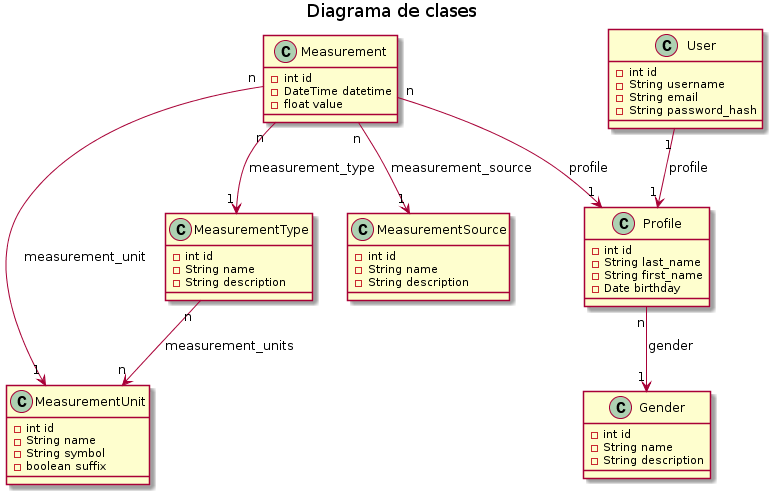
\includegraphics[width=.8\textwidth]{img/3-diagramaClases_relacionTipos}
	\caption{Diagrama de clases, donde se puede ver la relación entre el tipo de medición y la unidad.}
	\label{relacion_tipo}
\end{figure}


\subsubsection{Clase \texttt{MeasurementType}}

Esta clase nos permitirá nomenclar los tipos de medida existentes.
Hasta el momento, hemos contemplado:
\begin{itemize}
	\item Peso corporal.
	\item Dimensión corporal (por ejemplo, altura)
	\item Glucosa en sangre.
	\item Grasa corporal.
\end{itemize}
Existen ciertas medidas que contemplan dos valores.
Éstas serán agregadas en un sprint futuro.

\paragraph{Descripción de los atributos}
\begin{itemize}
	\item \textbf{id}: Identificador único del tipo de medición(tipo \texttt{int}).
	\item \textbf{name}: Nombre del tipo de medición (tipo \texttt{string}).
	\item \textbf{description}: Descripción del tipo de medición (tipo \texttt{string}).
\end{itemize}

\paragraph{Dirección del recurso}
\begin{lstlisting}[language=json,firstnumber=1]
<BASE URL>/measurement_types/{id}
\end{lstlisting}

\paragraph{Json generado por la API} 
\begin{lstlisting}[language=json,firstnumber=1]
{
"resource": 
{
"name": "Peso",
"description": "Peso corporal de la persona.",
"id": 1
}
}
\end{lstlisting}

\subsubsection{Clase \texttt{MeasurementUnit}}

Esta clase nos permitirá nomenclar las unidades de medición disponibles, para que el usuario pueda seleccionarlas cuando realice la medición.
Hasta el momento, hemos contemplado:
\begin{itemize}
	\item Kilogramo (Kg).
	\item Gramo (g).
	\item Miligramo (mg).
	\item Metro (m).
	\item Centímetro (cm).
	\item Milímetro (mm).
	\item Porcentaje (\%).
\end{itemize}

\paragraph{Descripción de los atributos}
\begin{itemize}
	\item \textbf{id}: Identificador único de la unidad de medición(tipo \texttt{int}).
	\item \textbf{name}: Nombre de la unidad de medición ( tipo \texttt{string}).
	\item \textbf{symbol}: Símbolo de la unidad de medición (tipo \texttt{string}).
	\item \textbf{suffix}: Variable booleana que indica si el símbolo de la unidad de medición es un sufijo (\textit{verdadero}) o un prefijo (\textit{falso}) del valor de la medición (tipo \texttt{boolean}).
\end{itemize}

\paragraph{Dirección del recurso}
\begin{lstlisting}[language=json,firstnumber=1]
<BASE URL>/measurement_units/{id}
\end{lstlisting}

\paragraph{Json generado por la API} 
\begin{lstlisting}[language=json,firstnumber=1]
{
"resource": 
{
"symbol": "Kg",
"suffix": true,
"name": "Kilogramo",
"id": 1
}
}
\end{lstlisting}


\subsubsection{Relación entre \texttt{MeasurementType} y \texttt{MeasurementUnit}}

Fundamentalmente, necesitamos el recurso que nos permite conocer las unidades de medidas a partir de un tipo de medición particular.
Dicho recurso provee la información necesaria para determinar las unidades de medida válidas, para un tipo de medición.

\paragraph{Dirección del recurso}
\begin{lstlisting}[language=json,firstnumber=1]
<BASE URL>/measurement_types/{id}/units
\end{lstlisting}

\paragraph{Json generado por la API} 

Retorna la lista de unidades de medición relacionadas a un tipo de medición específico.

\begin{lstlisting}[language=json, caption=Json generado por la api, label=unitPeso]
{
"resource": 
[{
"id": 1,
"symbol": "Kg",
"suffix": true,
"name": "Kilogramo"
},
{
"id": 6,
"symbol": "g",
"suffix": true,
"name": "gramo"
}]
}
\end{lstlisting}


\subsection{Ejecución de pruebas}

A continuación, se detalla la situación en la que quedaron las pruebas ejecutadas en los sprint anteriores.
Luego, se desarrollan las soluciones que se implementaron y, por último, se cambia el estado de aquellos errores encontrados, por el estado \textit{``Cerrado''}.

\subsubsection{Estado inicial de pruebas}

	\begin{itemize}
		\item \textbf{¿Qué fue bien?}
        	\begin{itemize}
				\item Las cargas y ediciones se llevan a cabo correctamente.
			\end{itemize}

   		\item \textbf{¿Qué se mejoró?}
        	\begin{itemize}
				\item \textbf{Cerrado}: Al crear una nueva medición, se mostraba un cartel (\textit{alert} de JavaScript) con una fecha. Dicho \textit{alert} fue eliminado.
                \item \textbf{Cerrado}: Se encontró un problema con la zona horaria que usa el servidor y la zona horaria del usuario. Para solucionarlo, hubo que hacer una conversión de fecha y hora previa, cuando se solicitaba la fecha y hora del usuario para mostrar.
			\end{itemize}

   		\item \textbf{¿Qué se puede mejorar?}
        	\begin{itemize}
		        \item \textbf{Abierto}: Sólo deberían mostrarse las unidades relacionadas al tipo de medición que se ha seleccionado.
				\item \textbf{Abierto}: En el futuro, se deberán mejorar las validaciones de los datos a la hora de cargar información en los formularios.
        		\item \textbf{Abierto}: Se deberá mejorar la manera de seleccionar la fecha y la hora. 
                \item \textbf{Abierto}: Deberán implementarse los carteles de advertencia necesarios.
            \end{itemize}
       
	\end{itemize}

\subsubsection{Correcciones efectuadas}

\paragraph{Mostrar unidades relacionadas al tipo de medición seleccionado}

Para evitar errores humanos, fue necesario mostrar sólo las unidades de medida que se encuentran relacionadas al tipo de medición seleccionado por el usuario.
Por ejemplo: si selecciona \textbf{Tipo de medición: ``\textit{Peso}''}, como se muestra en la \textbf{Figura \ref{unidad_peso}}, el sistema sólo debería mostrar las unidades que correspondan a ese tipo de medición, y no mostrar, por ejemplo, ``Metros'' como una posible unidad. Lo mismo se presenta para el caso de que seleccione la ``Altura'' como tipo de medición, como se observa en la \textbf{Figura \ref{unidad_altura}}.

A nivel de Front-end, fue necesario deshabilitar la selección de unidades cuando el usuario no ha seleccionado el tipo de medición, como se indica en la \textbf{Figura \ref{msj_seleccione_tipo}}.
Una vez seleccionado, se tuvo que solicitar a un recurso de la API las unidades relacionadas al tipo de medición, como se muestran en las figuras antes citadas.

 
 \begin{figure}[h]
  \centering
  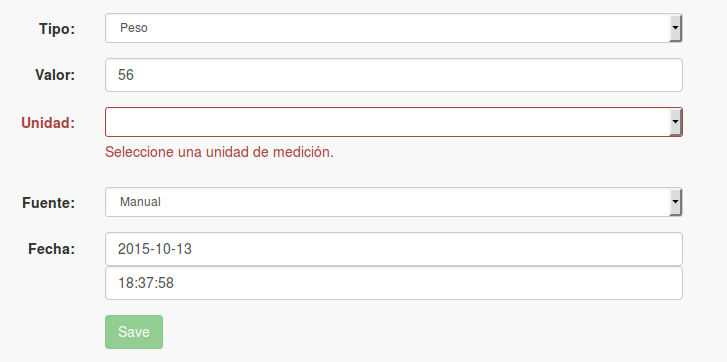
\includegraphics[width=.8\textwidth]{img/3-selecciona_tipo}
  \caption{Mensaje que solicita la selección de un tipo de medición.}
  \label{msj_seleccione_tipo}
\end{figure}

\begin{figure}[h]
  \centering
  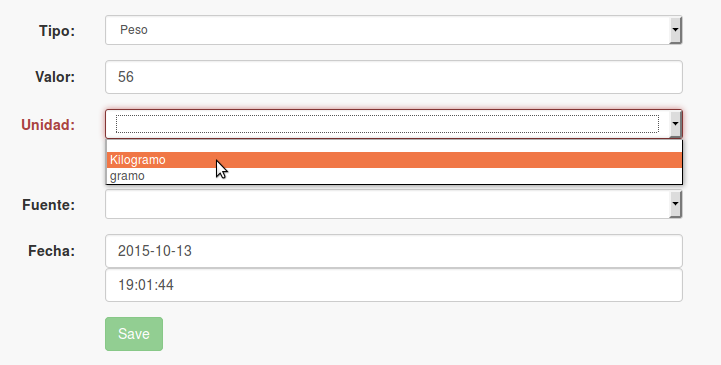
\includegraphics[width=.8\textwidth]{img/3-unidad_peso}
  \caption{Lista de unidades, al seleccionar el tipo de unidad ``Peso''.}
  \label{unidad_peso}
\end{figure}

 \begin{figure}[h]
  \centering
  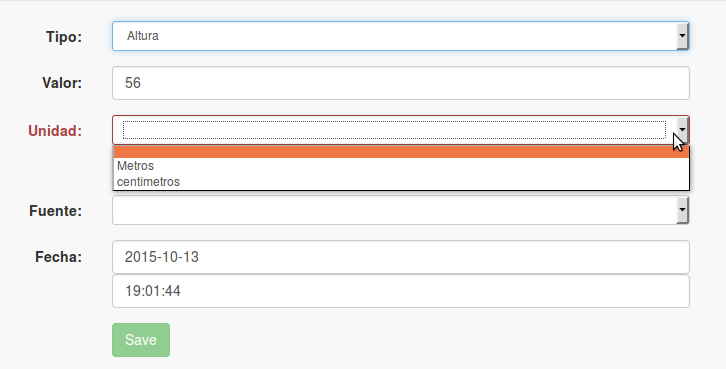
\includegraphics[width=.8\textwidth]{img/3-unidad_altura}
  \caption{Lista de unidades, al seleccionar el tipo de unidad ``Altura''.}
  \label{unidad_altura}
\end{figure}

\clearpage

El diagrama de clases, las relaciones y los recursos de la API necesarios para poder establecer esta relación, se detallan en la \textbf{Sección \ref{3-clases_involucradas}}.

El recurso implementado, que controla la solicitud de unidades de medición propias de un tipo de medición, se detalla en \textbf{Listing \ref{type_unit}}.

\begin{lstlisting}[language=JavaScript, caption=Recurso que solicita las unidades de un tipo de medición específico., label=type_unit]

angular.module('saludWebApp')                                                   
.factory('MeasurementTypeUnit', function (global, $resource) {                  
// URL of specific API resource                                             
var url=global.getApiUrl()+'/measurement_types/:id_type/units'; 

return $resource( url,                                                      
{ id_type: '@_id_type' },                                                        
{ query:{method:'GET',isArray:false},                                   
update: {method: 'PUT'}                                               
});                                                                     
});
\end{lstlisting}



\paragraph{Carteles de alerta}

Luego de ejecutar las pruebas, se detectó que para mejorar la experiencia del usuario es necesario añadir mensajes de avisos, como se muestra en las \textbf{Figuras \ref{msj_presiona_no_escribe}} y \textbf{\ref{msj_escribir_borrar}}, indicando al usuario situaciones importantes, como las que indican ausencia de información relevante en el formulario.
Además, el botón para enviar el formulario se mantiene deshabilitado hasta que se hayan completado los datos obligatorios (en este caso, todos los campos) del formulario.


 \begin{figure}[h]
  \centering
  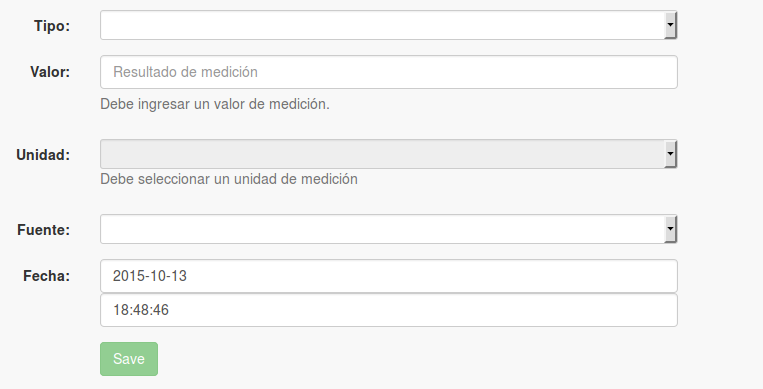
\includegraphics[width=.8\textwidth]{img/3-presiona_no_escribe}
  \caption{Mensaje sutil que aparece si se ha presionado el campo y no se ha escrito nada.}
  \label{msj_presiona_no_escribe}
\end{figure}

\begin{figure}[h]
  \centering
  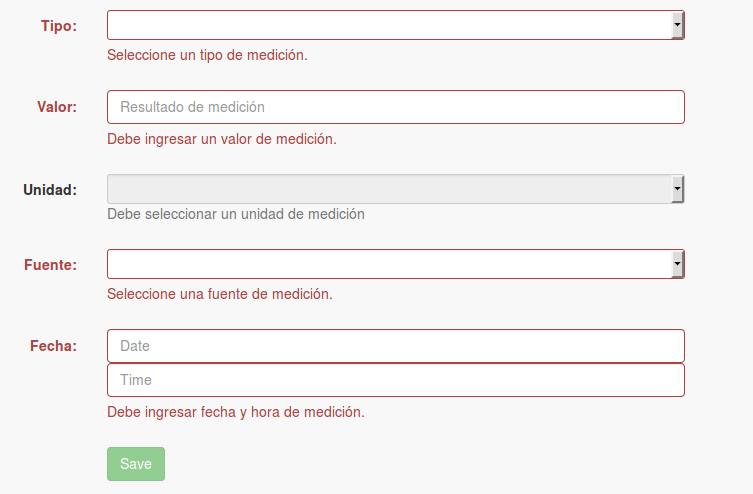
\includegraphics[width=.8\textwidth]{img/3-escribir_borrar}
  \caption{Mensaje vistoso que aparece luego de borrar lo escrito.}
  \label{msj_escribir_borrar}
\end{figure}

\clearpage

\paragraph{Variable de acceso a la API global}

Fue necesario añadir un servicio para manejar la dirección global de la API, para facilitar su parametrización, en caso de que la misma se modifique.

Dicho servicio se detalla en \textbf{Listing \ref{direccion_global}}.

\begin{lstlisting}[language=JavaScript, caption=Servicio de la dirección global de la API, label=direccion_global]
'use strict';                                                                   
                                                                                
/**                                                                             
 * @ngdoc service                                                               
 * @name saludWebApp.global                                                     
 * @description                                                                 
 * # global                                                                     
 * Factory in the saludWebApp.                                                  
 */                                                                             
angular.module('saludWebApp')                                                   
  .factory('global', function () {                                              
    // Service logic                                                               
                                                                                
    // URL of yesdoc API                                                           
    var _api_url='https://yesdoc-api.herokuapp.com';                               
                                                                                   
    // Public methods                                                              
    return {                                                                       
      getApiUrl: function () {                                                     
        return _api_url;                                                           
      }                                                                            
    };                                                                             
  });                                                       
\end{lstlisting}


\subsubsection{Estado final de pruebas}

	\begin{itemize}
		\item \textbf{¿Qué fue bien?}
        	\begin{itemize}
				\item Las cargas y ediciones se llevan a cabo correctamente.
			\end{itemize}

   		\item \textbf{¿Qué se mejoró?}
        	\begin{itemize}
				\item \textbf{Cerrado}: Al crear una nueva medición, se mostraba un cartel (\textit{alert} de JavaScript) con una fecha. Dicho \textit{alert} fue eliminado.
                \item \textbf{Cerrado}: Se encontró un problema con la zona horaria que usa el servidor y la zona horaria del usuario. Para solucionarlo, hubo que hacer una conversión de fecha y hora previa, cuando se solicitaba la fecha y hora del usuario para mostrar.
			\end{itemize}

        	\begin{itemize}
		        \item \textbf{Cerrado}: Sólo deberían mostrarse las unidades relacionadas al tipo de medición que se ha seleccionado.
		        \item \textbf{Cerrado}: En el futuro, se deberán mejorar las validaciones de los datos a la hora de cargar información en los formularios.
		        \item \textbf{Cerrado}: Se deberá mejorar la manera de seleccionar la fecha y la hora. 
		        \item \textbf{Cerrado}: Deberán implementarse los carteles de advertencia necesarios.
            \end{itemize}
	\end{itemize}